\documentclass[crop,tikz]{standalone}
\usetikzlibrary{backgrounds}
\colorlet{blue}{cyan}
\tikzset{
  inverted/.style = {
    color=white,
    background rectangle/.style={fill},
    show background rectangle
  }
}

\usepackage{amsmath}
\usepackage{pgfplots}
\tikzset{>=latex}
\colorlet{green}{green}

\pgfplotsset{
  every non boxed x axis/.append style={
    axis line style={-latex}
  },
  every non boxed y axis/.append style={
    axis line style={-latex}
  },
  inverted/.style = {
    every axis legend/.append style={
      draw=white,
      fill=white,
      text=white
    }
  }
}

\begin{document}
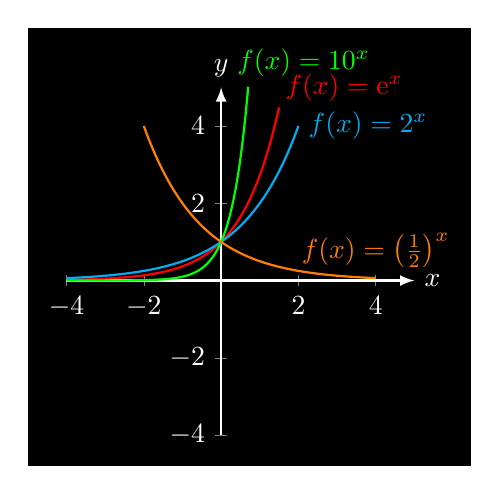
\begin{tikzpicture}[inverted,inverted]
\begin{axis}[inverted,
  thick,
  width=6cm,
  height=6cm,
  samples=100,
  smooth,
  axis y line=middle,
  axis x line=middle,
  xlabel={$x$},
  ylabel={$y$},
  xlabel style={right},
  ylabel style={above},
  xmin=-4, xmax=5,
  ymin=-4, ymax=5,
  clip=false,
  ]
  \addplot[red,smooth,domain=-4:1.5] { exp(x) };
  \node[red,right] at (axis cs:1.4,5) {$f(x)=\operatorname{e}^x$};
  \addplot[blue,smooth,domain=-4:2] { 2^x } node[right] {$f(x)=2^x$};
  \addplot[green,smooth,domain=-4:0.7] { 10^x } node[above,xshift=2em] {$f(x)=10^x$};
  \addplot[orange,smooth,domain=-2:4] { 0.5^x } node[above] {$f(x)=\left(\frac{1}{2}\right)^x$};
\end{axis}
\end{tikzpicture}
\end{document}
